% @Author: AnthonyKenny98
% @Date:   2020-04-05 20:05:17
% @Last Modified by:   AnthonyKenny98
% @Last Modified time: 2020-04-05 20:55:20

\begin{figure}[H]
\begin{centering}
\begin{tabular}{cc}

    \begin{subfigure}{0.5\linewidth}
    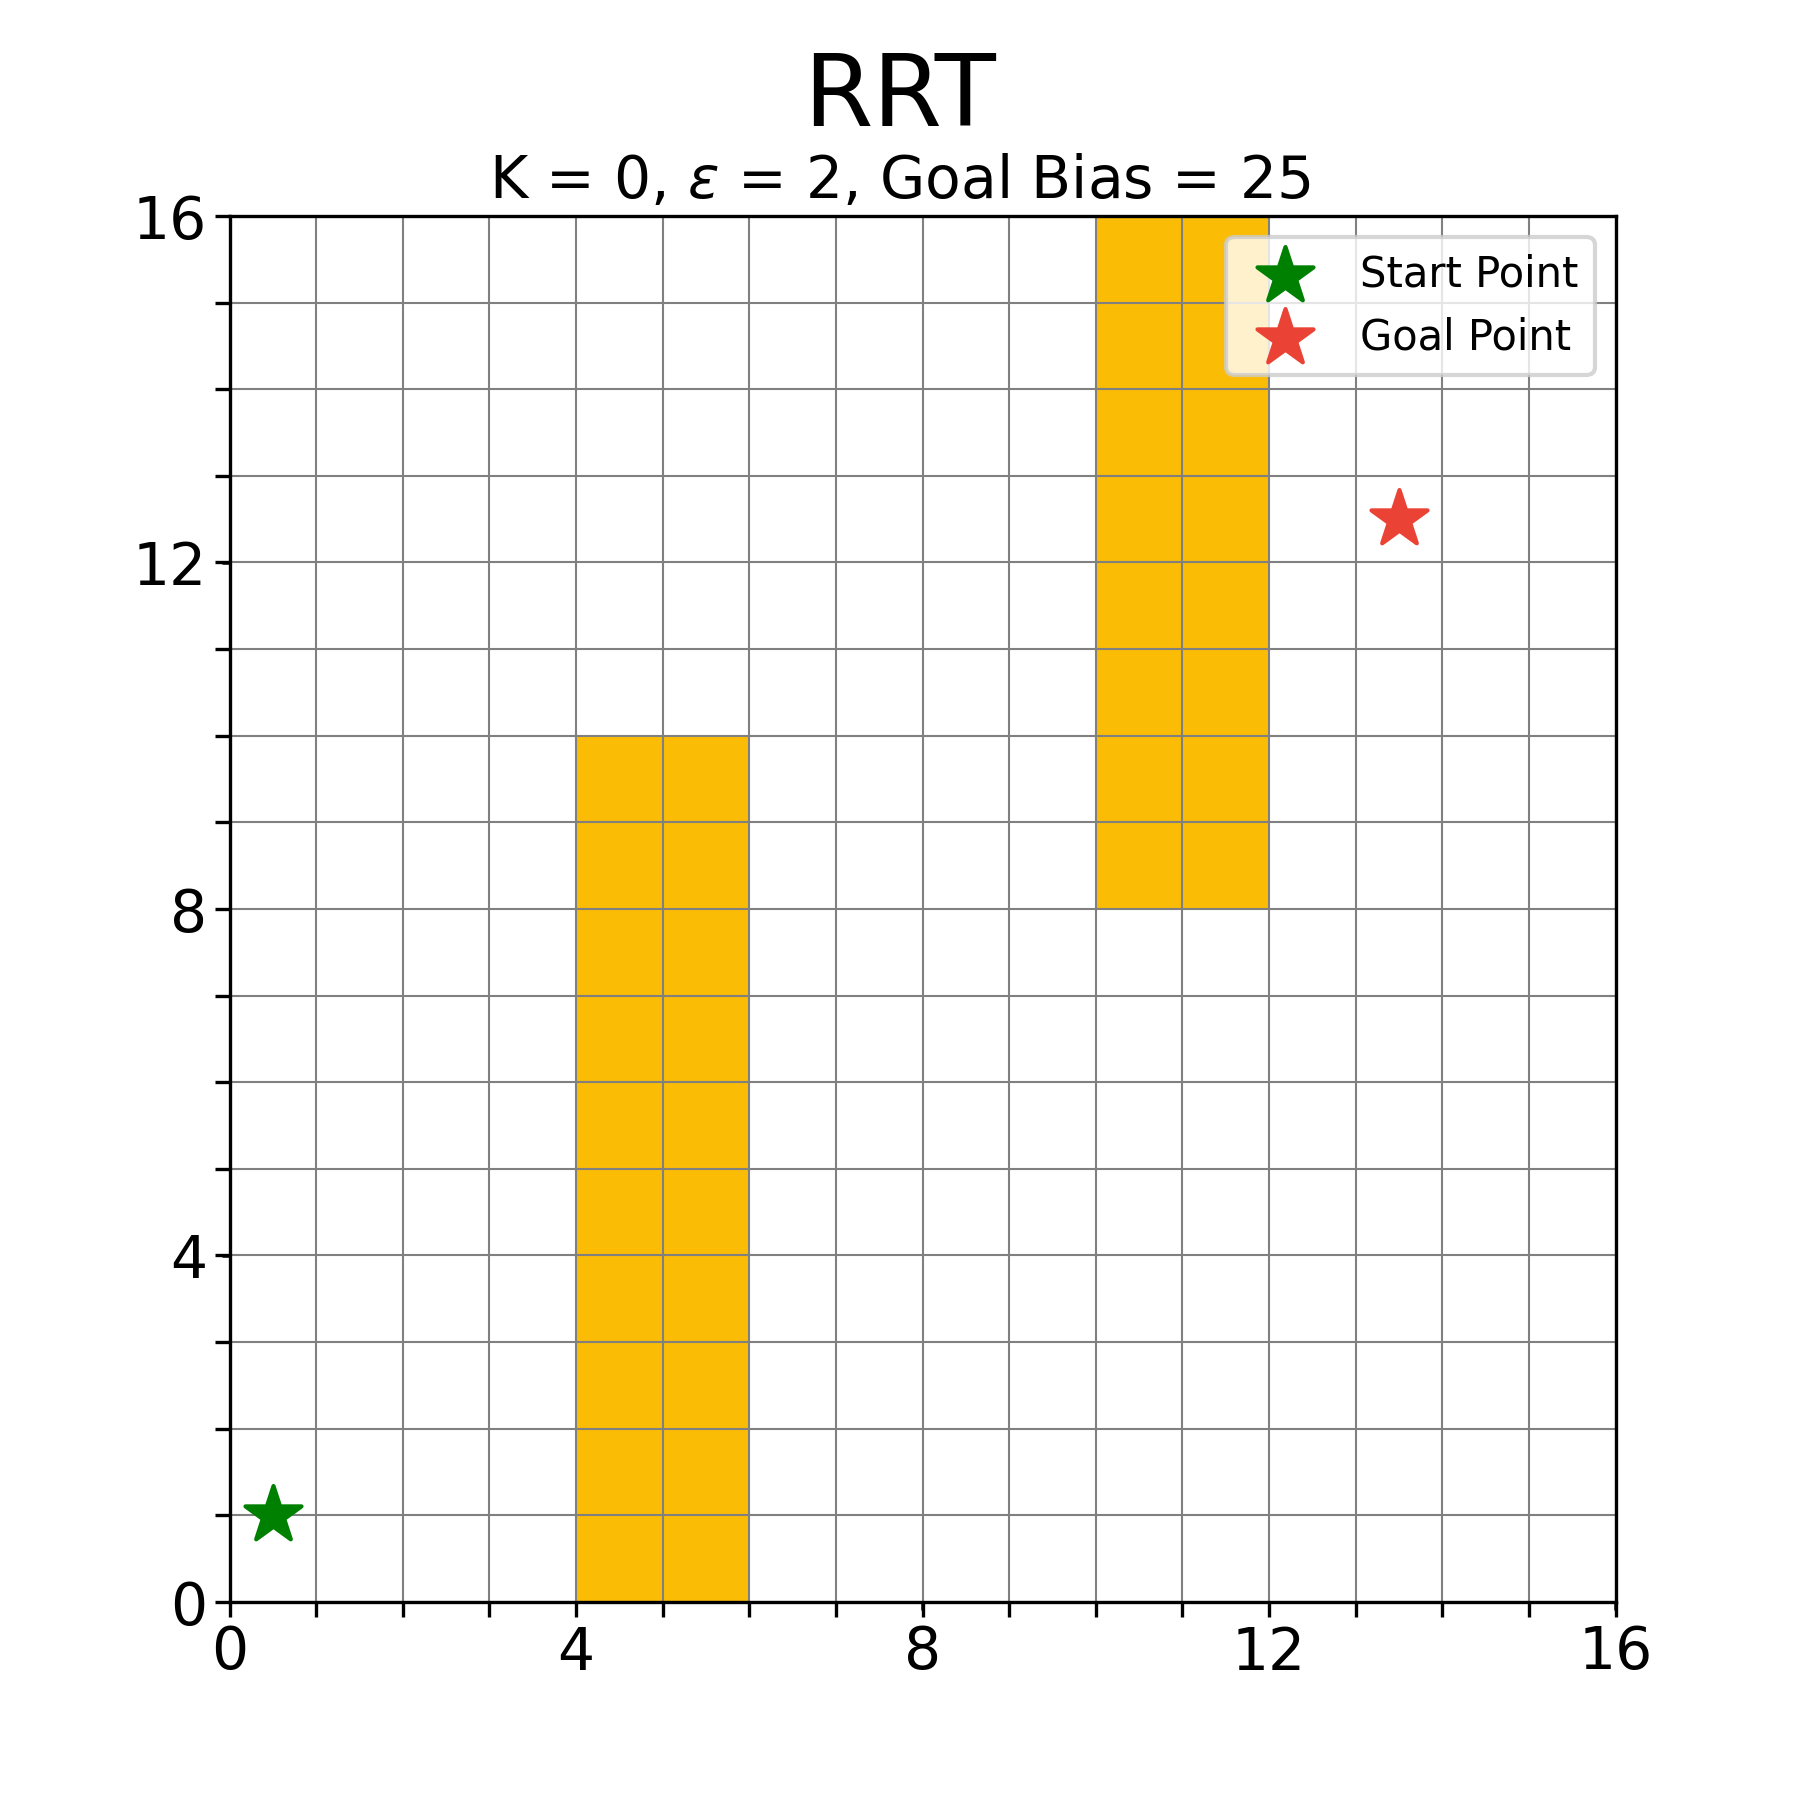
\includegraphics[width=\linewidth]{chapters/chapter2/img/visualizing/obstacles2d.png}
    \caption{Obstacles in 2D}
    \end{subfigure} &

    \begin{subfigure}{0.5\linewidth}
    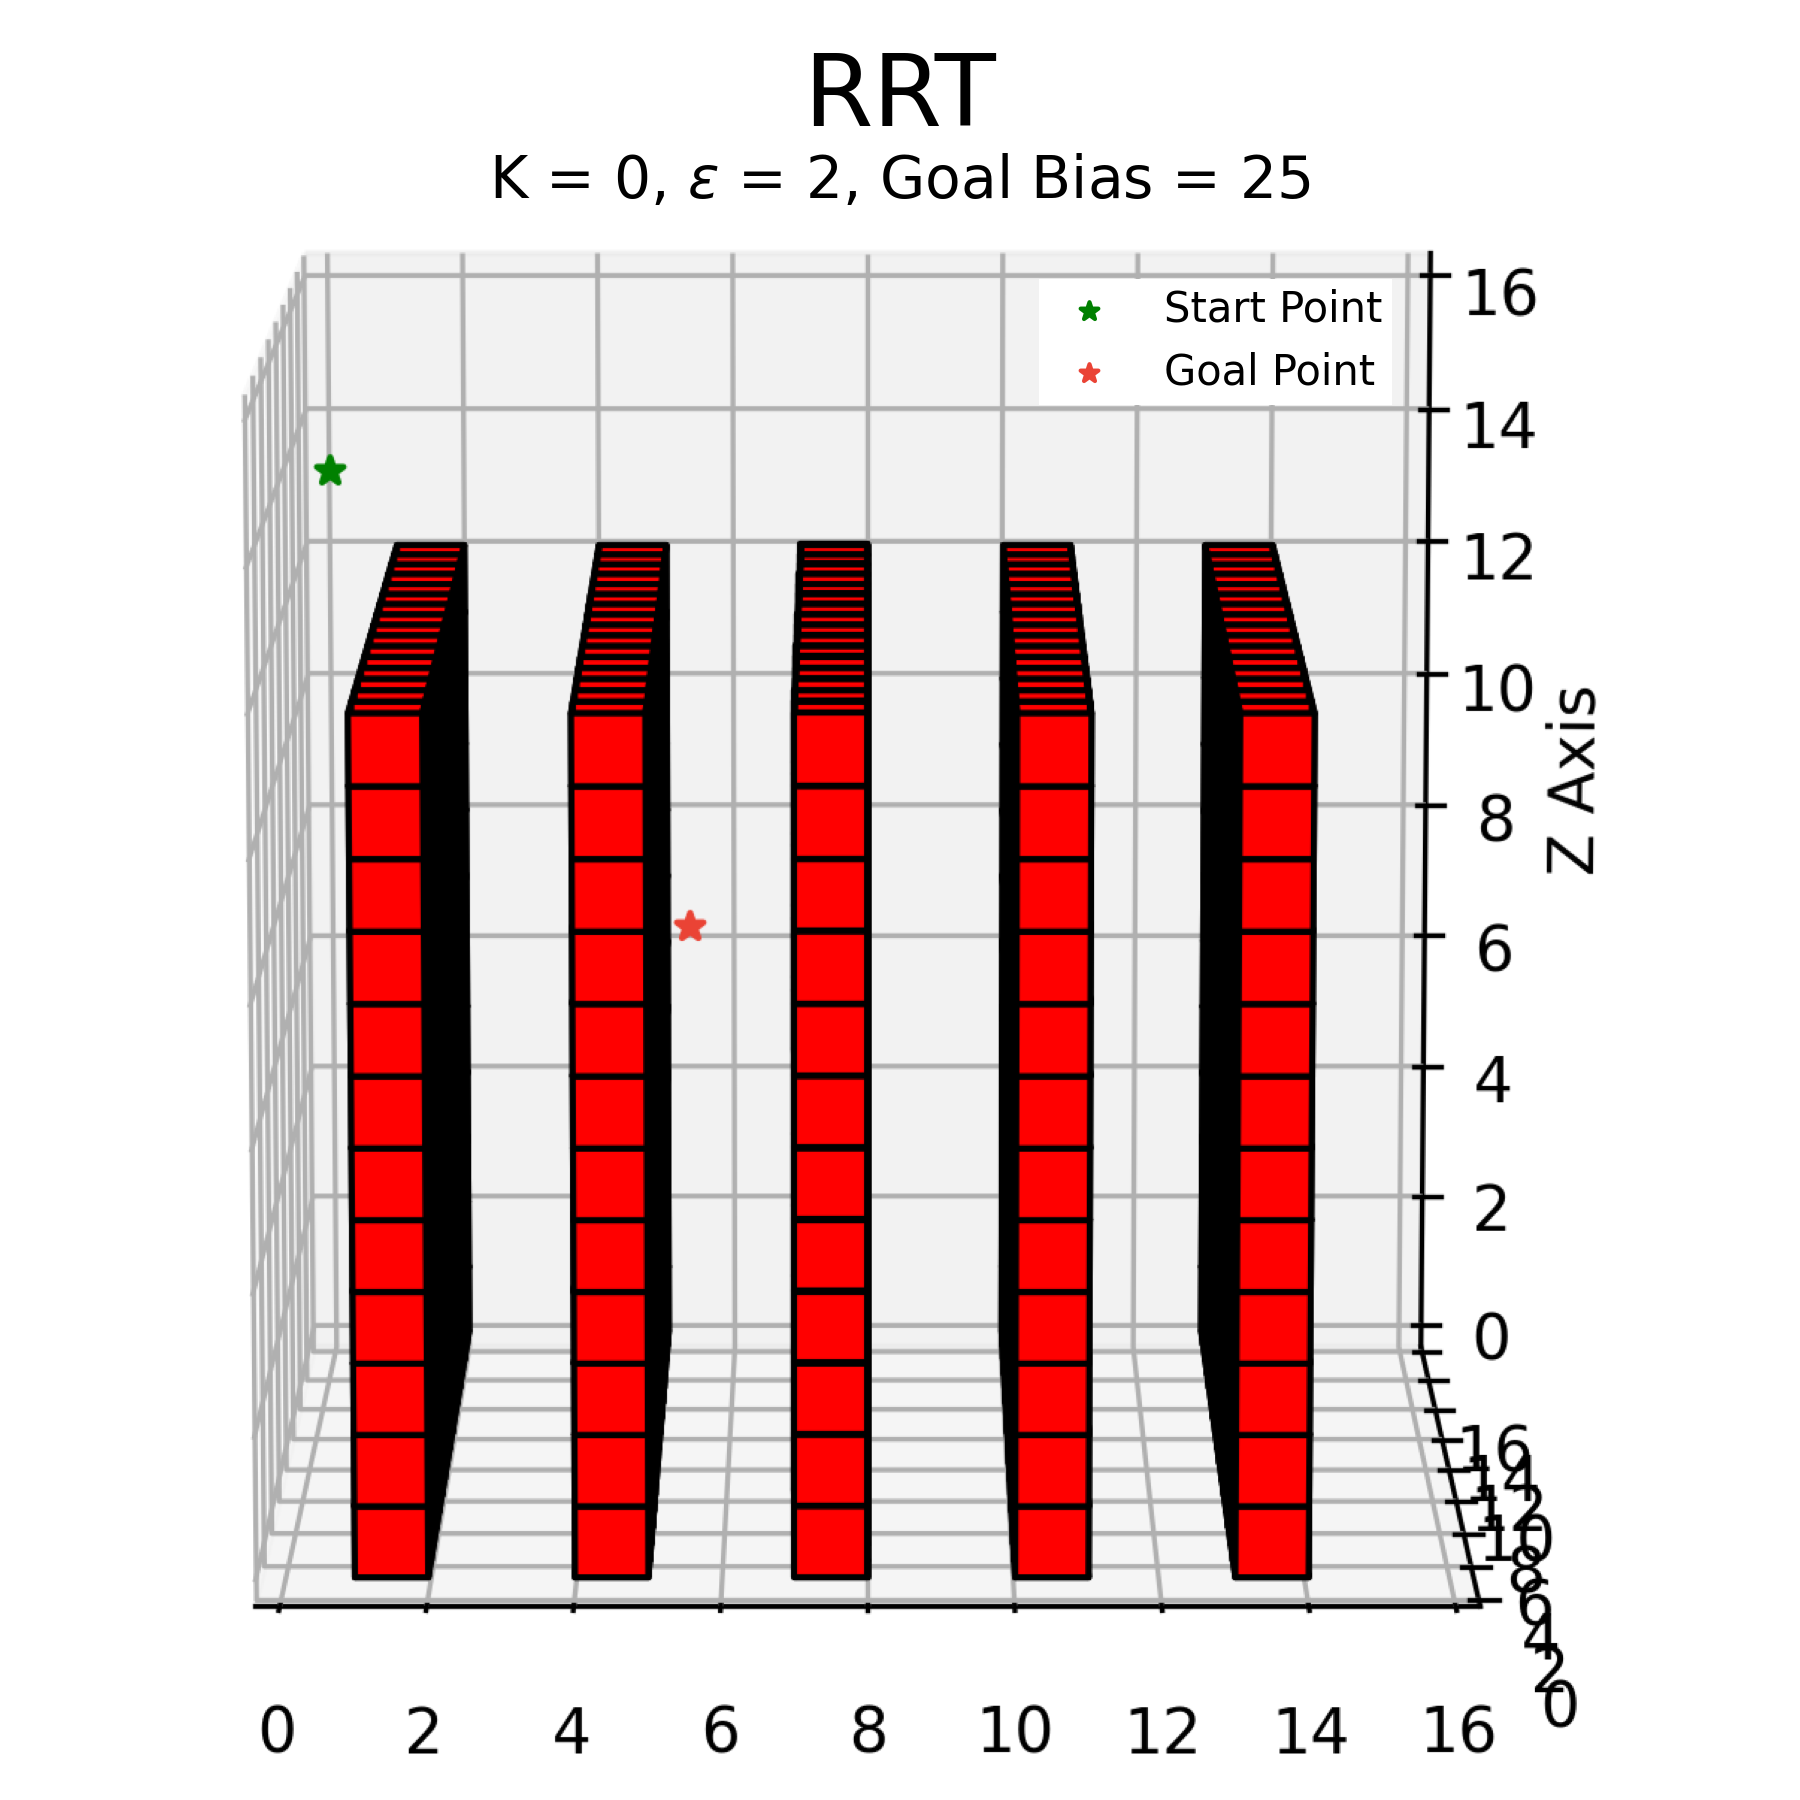
\includegraphics[width=\linewidth]{chapters/chapter2/img/visualizing/obstacles3d.png}
    \caption{Obstacles in 3D}
    \end{subfigure} \\

\end{tabular}
\caption[Visualization of Obstacles in 2D and 3D]{\textbf{Visualization of Obstacles in 2D and 3D}, Obstacles shown in yellow and red for 2D and 3D respectively.}
\label{fig:rrt_obstacles}
\end{centering}
\end{figure}